\documentclass[../file_doc_script.tex]{subfiles}
\usepackage[french]{babel}
\usepackage{listings}
\usepackage{subfiles}
\usepackage{graphicx}
\usepackage[utf8]{inputenc}
\usepackage{fancyhdr}
\usepackage{tabularx}
\usepackage{listings}
\usepackage{float}
\usepackage{xcolor}

\begin{document}

\section{Utilisation des scripts}
Tous les scripts dévellopés dans le cadre de ce projet possède une documentation,
qui est l'éuivalent d'un manuel. Pour y avoir accès il suffit de taper le nom du script
tout seul et une documentation s'affichera.

\subsection{Utilisation du script dans un terminal}
\begin{figure}[h]
    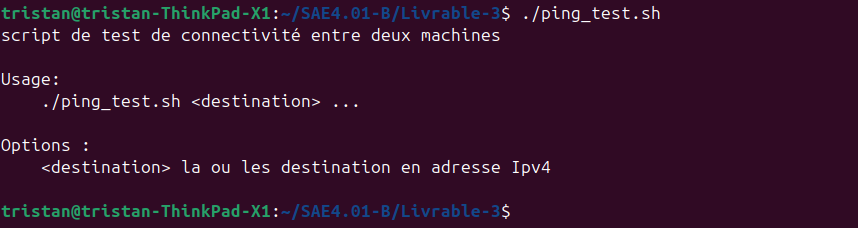
\includegraphics[width=1\textwidth]{../Images/doc-script-terminal.png}
    \caption{Manuel d'utilisation du script}
    \label{fig:solution1}
\end{figure}

\subsection{Implémentation de cette documentation}
Pour cette documentation, nous avons inclus un if pour détecter si aucun paramètre n'a été 
donné au script. Dans ces cas là il lève une erreur en montrant les options que peut utiliser 
l'administrateur pour ce script.

\UseRawInputEncoding
\lstinputlisting[firstline=7,lastline=19, caption= extrait de la doc du script de ping]{../ping_test.sh}


\end{document}
